% **** Szablon pracy magisterskiej, licencjackiej lub inżynierskiej ****

\documentclass[polish,12pt,twoside,a4paper]{report}

\input{style.tex}

%definicja przydatnych poleceń
\newcommand{\wydzial}{KOLEGIUM INFORMATYKI STOSOWANEJ}
\newcommand{\kierunek}{Kierunek: INFORMATYKA}
\newcommand{\specjalnosc}{Grupa: 3IIZ/2024/25 GL04 }
\newcommand{\autor}{Tomasz Cisło}
\newcommand{\album}{Nr albumu studenta w65678, 3IIZ/GL04}
\newcommand{\temat}{Aplikacja z możliwością nadania przesyłek}
\newcommand{\promotor}{Mgr inż. Ewa Żesławska}
\newcommand{\typpracy}{Programowanie obiektowe C\# - Projekt}
\newcommand{\miasto}{Rzeszów}
\newcommand{\rok}{2025}

\begin{document}

% *************** Włączenie definicji pierwszych stron ***************
\input{front.tex}


% *************** Część główna pracy ***************
\setcounter{section}{0}
\renewcommand{\thesection}{\arabic{section}}

\section{Założenia}
\subsection{Cel aplikacji}

Aplikacja PocztaExpress została stworzona w celu uproszczenia procesu nadawania paczek. Umożliwia użytkownikom szybkie i wygodne wypełnienie formularza nadawczego. Głównym celem aplikacji jest eliminacja potrzeby osobistego odwiedzania placówek pocztowych, co przekłada się na oszczędność czasu i zwiększenie wygody użytkownika.

\subsection{Zastosowanie}

Aplikacja może być wykorzystywana przez:
\begin{itemize}
\item Klientów indywidualnych, którzy chcą nadać paczkę bez wychodzenia z domu
\item Firmy i sklepy internetowe do usprawnienia procesu wysyłki zamówień
\item Kurierów oraz placówki logistyczne do zarządzania przesyłkami
\end{itemize}

\subsection{Wymagania funkcjonalne}
\begin{itemize}
\item Logowanie oraz rejestracja konta
\item Rejestrowanie przesyłek 
\item Wyświetlanie historii przesyłek
\item System dodawania punktów do użytkownika
\item Zmiana hasła dla zalogowanego użytkownika
\item Możliwość dodania komentarzy 
\item Zmiana ceny dla nadania przesyłki
\end{itemize}

\subsection{Wymagania niefunkcjonalne}
\begin{itemize}
\item Wydajność
\item Aplikacja w pełni kompatybilna z systemami Windows 10/11
\item Aplikacja stworzona z intuicyjnym interfejsem
\end{itemize}
\newpage
\section{Struktura projektu}
\subsection{Wykorzystanie języka}
Aplikacja PocztaExpress została zaprojektowana przy użyciu języka programowania C\# w oparciu o platformę .NET 8.0. Interfejs użytkownika zbudowano w technologii Windows Forms, co zapewnia wygodną obsługę i prostotę w nawigacji. 
\subsection{Wymagania sprzętowe}
Minimalne wymagania sprzętowe dla aplikacji obejmują komputer wyposażony w procesor Intel Core i3 lub jego odpowiednik od AMD. Zalecana ilość pamięci RAM to co najmniej 4 GB, aby zapewnić płynną pracę programu. Aplikacja wymaga także co najmniej 40 MB wolnego miejsca na dysku twardym w celu przechowywania plików
\subsection{Baza danych}
Aplikacja korzysta z relacyjnej bazy danych SQL Server, w której przechowywane są wszystkie dane dotyczące użytkowników i przesyłek. Baza danych zawiera dwie główne tabele. Pierwszą z nich jest tabela users, która przechowuje informacje o użytkownikach, takie jak identyfikator, imię, nazwisko, adres e-mail, hasło. Drugą kluczową tabelą jest historia\verb|_|wysylek, która rejestruje wszystkie informacje dotyczące nadanych paczek. Każda przesyłka ma przypisany unikalny identyfikator. Następną tabelą jest cennik, który przechowuje aktualne ceny kosztów nadania przesyłki. Kolejną jest tabela punkty która przechowuje punkty użytkownika. Następną są komentarze przechowujące informacje od różnych użytkowników. Zarządzanie danymi odbywa się poprzez bezpośrednie zapytania SQL wykonywane przez kod aplikacji. Używane są instrukcje SELECT do pobierania informacji o przesyłkach i użytkownikach, INSERT do dodawania nowych rekordów
\subsection{Diagram Klas}
Na rysunku 1 został przedstawiony diagram klas
\begin{figure}[!ht]
\centering
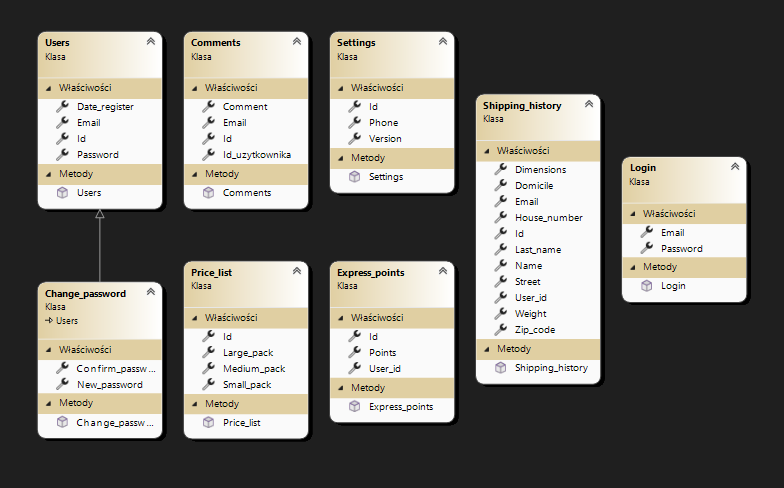
\includegraphics[width=17cm, height=8cm]{figures/diagram.png}
\caption{\footnotesize Diagram reprezentujacy klasy. }
\label{fig:plotend}
\end{figure}
\newpage
\subsection{Opis klas}
\begin{itemize}
\item \textit{Change\textunderscore password} – klasa odpowiedzialna za zmianę hasła z aktualnego na nowe
\item \textit{Comments} – klasa reprezentująca komentarze napisane przez użytkowników aplikacji (małe forum)
\item \textit{Express\textunderscore points} – klasa reprezentująca punkty za nadanie paczek
\item Login – Klasa służąca za zalogowanie się do aplikacji
\item Price\verb|_|list – Klasa odpowiedzialna za wyświetlanie aktualnych cen nadania paczki w zależności od rozmiaru paczki
\item Settings – Klasa reprezentująca ustawienia dla administratora aplikacji
\item Shipping\verb|_|history – Klasa odpowiedzialna za wyświetlenie informacji o przesyłkach już nadanych
\item Users – Klasa przechowująca listę użytkowników
\end{itemize}

\newpage
\section{Harmonogram realizacji projektu}

\begin{figure}[!ht]
	\centering
	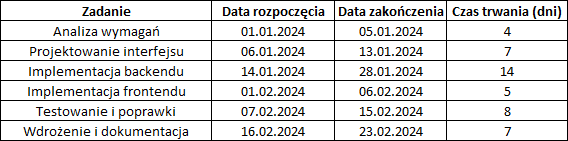
\includegraphics{figures/harmonogram.png}
	\caption{\footnotesize Harmonogram realizacji projektu - tabela. }
	\label{fig:plotend}
\end{figure}

\begin{figure}[!ht]
	\centering
	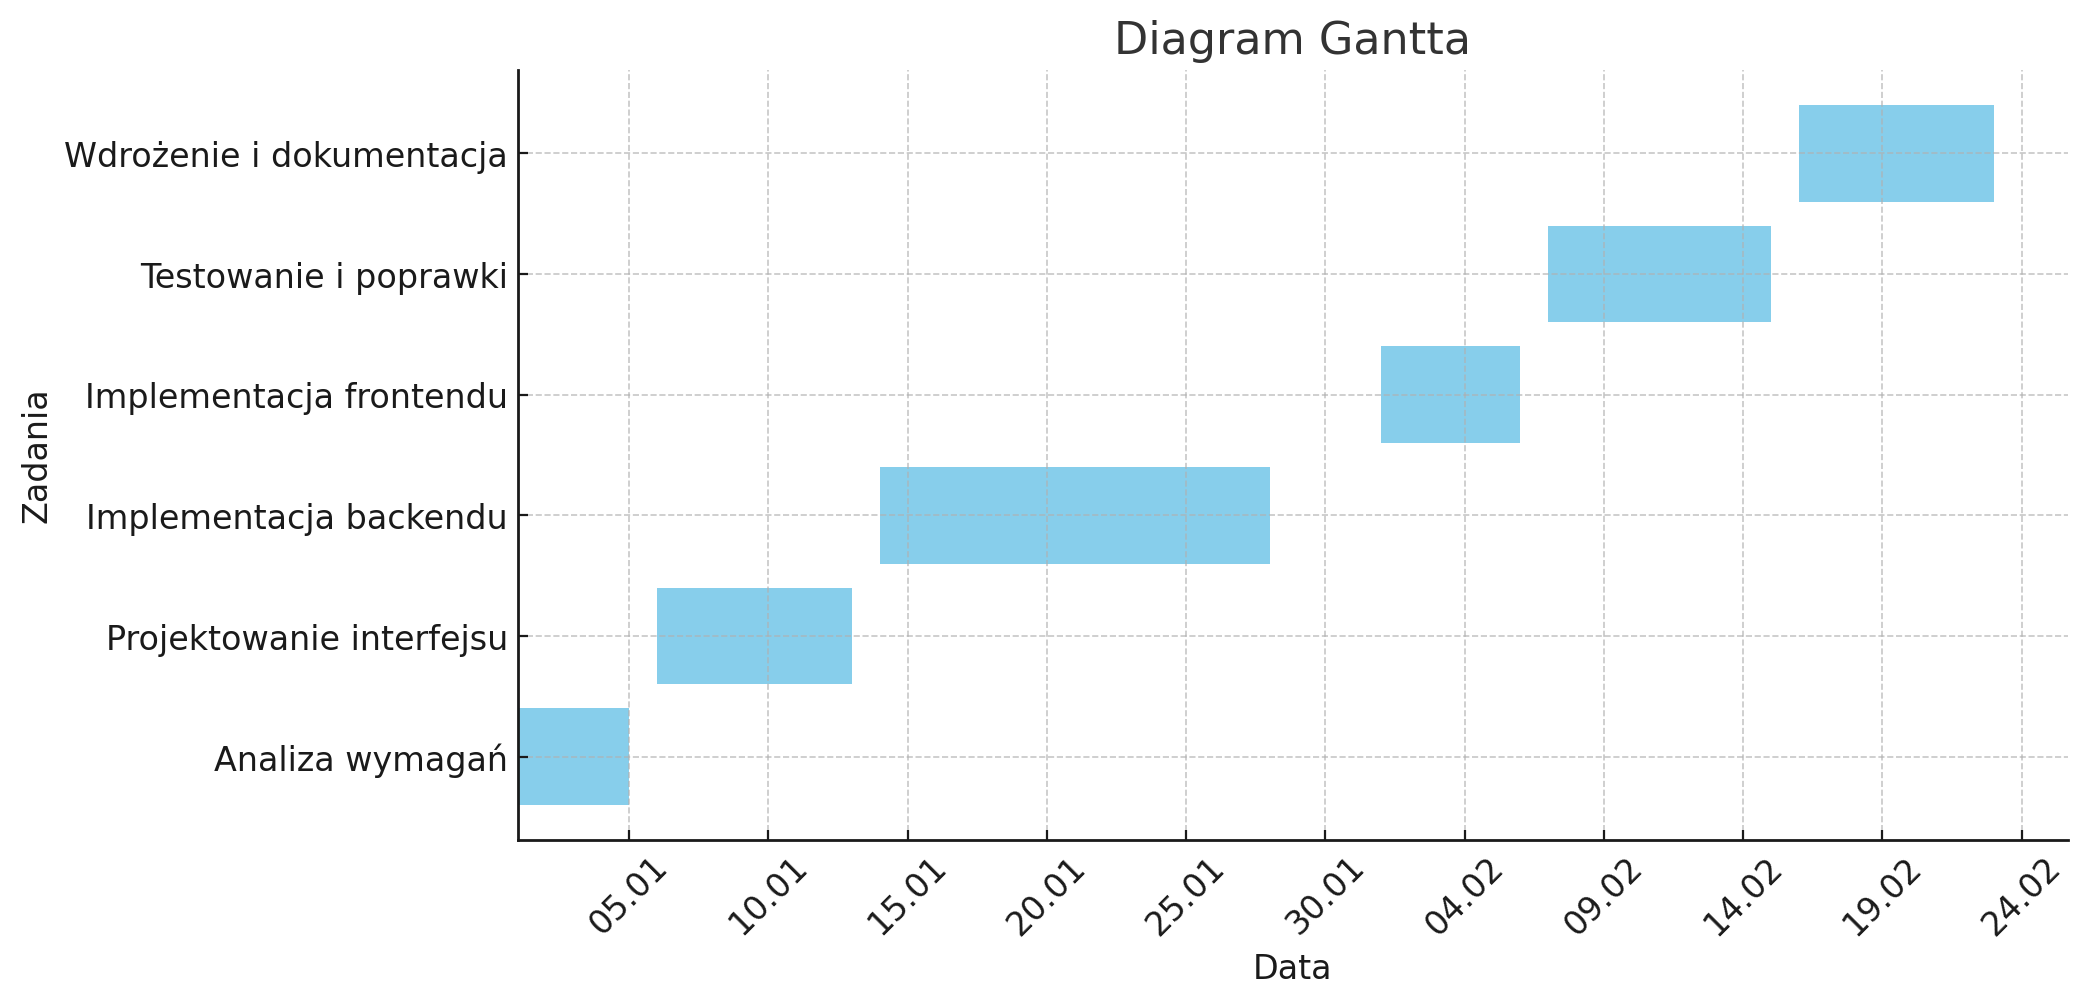
\includegraphics[width=17cm, height=8cm]{figures/diagram ganta.png}
	\caption{\footnotesize Harmonogram realizacji projektu - diagram Gantta. }
	\label{fig:plotend}
\end{figure}

\section{Repozytorium i system kontroli wersji}

Projekt zarządzany jestem w systemie kontroli wersji Git. 
\newline
Pod adresem \textit{https://github.com/tomaszcislo/projekt} dokumentowane są wszystkie zmiany
\newpage
\section{Warstwa użytkowa projektu}

Aplikacja PocztaExpress została stworzona w celu uproszczenia procesu nadawania paczek. Umożliwia użytkownikom szybkie i wygodne wypełnienie formularza nadawczego. Głównym celem aplikacji jest eliminacja potrzeby osobistego odwiedzania placówek pocztowych, co przekłada się na oszczędność czasu i zwiększenie wygody użytkownika.

\subsection{Logowanie}

W oknie logowania (Rysunek 4) użytkownik podaje swoje dane do logowania (login oraz hasło) wymagane do zalogowania się. Dodatkowo w polu tekstowym do podania swojego hasła można wyłączyć symbole zastępcze podczas gdy użytkownik wpisze ciąg swojego hasła. Po zaznaczeniu checkbox’a symbole zostaną wyłączone. Po wpisaniu hasła od użytkownika wymagane jest naciśnięcie przycisku „ZALOGUJ” w celu zalogowania się do aplikacji. Jeśli dane zostały poprawnie wpisane zostanie wyświetlony komunikat (Rysunek 5) o udanym zalogowaniu. W przypadku podania błędnych danych (loginu lub hasła) użytkownik nie zostanie zalogowany oraz zostanie wyświetlony komunikat  (Rysunek 6) o błędnym loginie lub haśle. Po naciśnięciu „OK” użytkownik będzie mógł poprawić swoje dane do logowania, a następnie podjąć próbę logowania ponownie.

\begin{figure}[!ht]
\centering
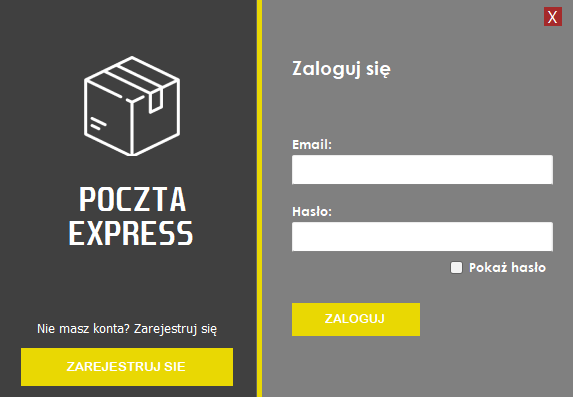
\includegraphics{figures/oknologowania.png}
\caption{\footnotesize Okno logowania. }
\label{fig:plotend}
\end{figure}



\begin{figure}[!ht]
\centering
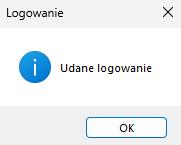
\includegraphics{figures/udane_logowanie.png}
\caption{\footnotesize Komunikat o pomyślnym zalogowaniu. }
\label{fig:plotend}
\end{figure}


\begin{figure}[!ht]
\centering
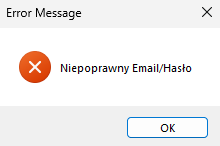
\includegraphics{figures/niepoprawny_email.png}
\caption{\footnotesize Komunikat o niepoprawnym zalogowaniu. }
\label{fig:plotend}
\end{figure}

\newpage

\subsection{Rejestracja}

W przypadku braku konta, użytkownik może stworzyć swoje konto klikając przycisk „ZAREJESTRUJ SIĘ” (Rysunek 7) Procedura rejestracji wygląda tak samo jak w przypadku logowania się. Po zarejestrowaniu się, użytkownik będzie mógł się zalogować



\begin{figure}[!ht]
\centering
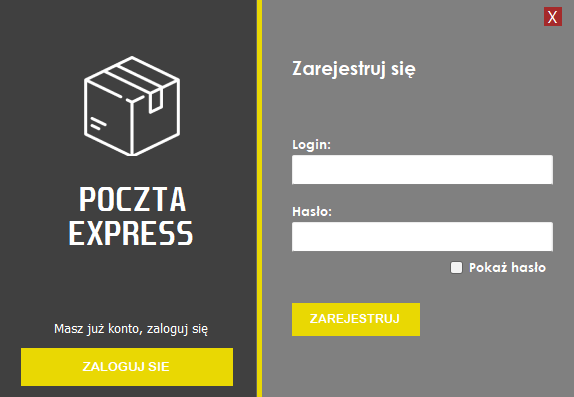
\includegraphics{figures/rejestracja.png}
\caption{\footnotesize Okno rejestracji. }
\label{fig:plotend}
\end{figure}

\newpage
\subsection{Nadanie przesyłki}

Rysunek 8 przedstawia okno do nadania paczki służy do nadania paczki przez nadawcę. W tym celu od nadawcy (użytkownika aplikacji) wymagane jest wprowadzenie do każdego pola tekstowego dane paczki oraz dane odbiorcy. Po uzupełnieniu wszystkich danych, aby paczka została nadana wymagane jest naciśnięcie przycisku o nazwie „NADAJ”.
W oknie również zaprezentowany jest cennik informujący o aktualnych cenach nadania paczki w zależności od jej rozmiaru

\begin{figure}[!ht]
\centering
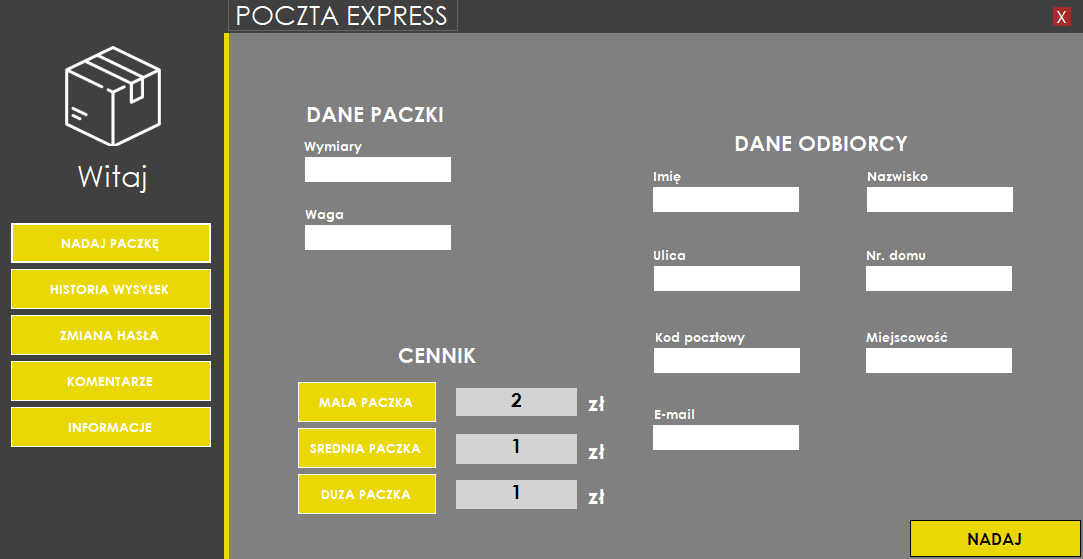
\includegraphics[width=16.5cm, height=9cm]{figures/okno_glowne.png}
\caption{\footnotesize Okno do nadania paczki. }
\label{fig:plotend}
\end{figure}

\noindent Po nadaniu paczki zostanie wyświetlony komunikat o pomyślnym nadaniu paczki (Rysunek 9)

\begin{figure}[!ht]
\centering

\includegraphics{figures/komunikat_o_poprawnym_nadaniu_paczki.png}
\caption{\footnotesize Komunikat o poprawnym nadaniu paczki. }
\label{fig:plotend}
\end{figure}

\noindent Okno główne aplikacji posiada menu boczne (Rysunek 10). Każdy przycisk odpowiada za otwarcie nowego okna zamykając aktualne. Menu boczne zostało zastosowane w każdym oknie ułatwiając przemieszczanie się do innych okien.

\begin{figure}[!ht]
\centering

\includegraphics{figures/menu_boczne.png}
\caption{\footnotesize Menu boczne. }
\label{fig:plotend}
\end{figure}

\noindent Menu boczne przedstawia następujące przyciski:

\begin{itemize}
\item Nadaj Paczkę – główne okno aplikacji – służy do nadania przesyłki wypełniając wcześniej formularz
\item Historia Wysyłek – wyświetla historię nadanych przez użytkownika przesyłek
\item Zmiana hasła – pozwala na zmianę hasła zalogowanego użytkownika
\item Komentarze – wyświetla możliwość udzielenia komentarza
\item Informacje – wyświetla informacje o aplikacji (np. wersja)
\end{itemize}

\newpage

\subsection{Historia wysyłek}

Po otworzeniu okna (Rysunek 11) zostanie wyświetlona lista prezentująca historię wysyłek wysłanych przez nadawcę (użytkownika)

\begin{figure}[!ht]
\centering
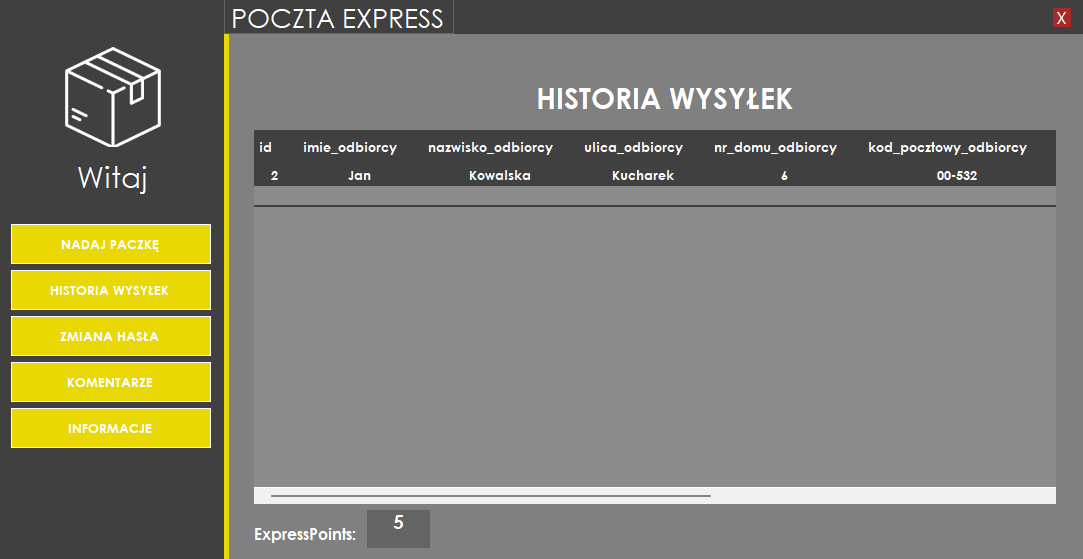
\includegraphics[width=16.5cm, height=9cm]{figures/okno_historiawysylek.png}
\caption{\footnotesize Okno przedstawiające listę wysłanych przesyłek przez nadawcę (użytkownika). }
\label{fig:plotend}
\end{figure}

\noindent Lista została stworzona za pomocą kontrolki DataGridView, który obsługuje standardowy model powiązania danych Windows Forms. Pobiera z bazy danych informację o wcześniej nadanych przesyłkach i je wyświetla. Lista historii jest przypisana do użytkownika. Dodatkowo wyświetla liczbę z punktami (ExpressPoints) które użytkownik posiada na swoim koncie. Punkty zdobywa się za nadanie paczek.

\begin{itemize}
\item Id – identyfikator przesyłki
\item Imie\verb|_|odbiorcy – imię odbiorcy
\item Nazwisko\verb|_|odbiorcy – nazwisko odbiorcy
\item Ulica\verb|_|odbiorcy – ulica odbiorcy
\item Nr\verb|_|domu\verb|_|odbiorcy – numer domu odbiorcy
\item Kod\verb|_|pocztowy\verb|_|odbiorcy – kod pocztowy odbiorcy
\item Miejscowosc – miejscowość odbiorcy
\item E-mail – e-mail odbiorcy
\item Wymiary - wymiary przesyłki
\item Waga - waga przesyłki
\end{itemize}


\subsection{Zmiana hasła}

Po otworzeniu okna (Rysunek 12) zostanie wyświetlony panel służący do zmiany aktualnego hasła

\begin{figure}[!ht]
\centering
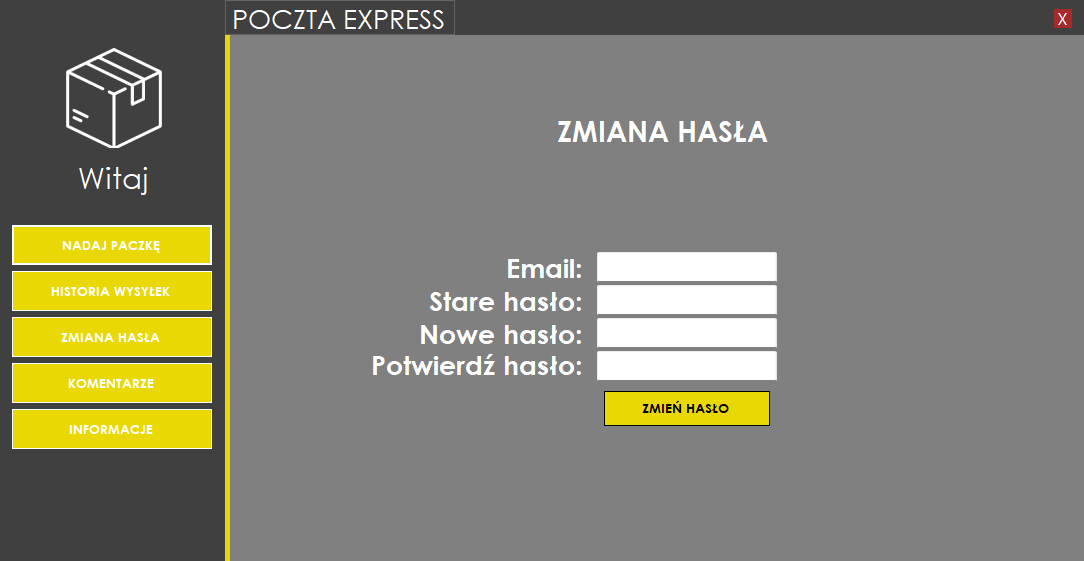
\includegraphics[width=16.5cm, height=9cm]{figures/zmiana_hasla.png}
\caption{\footnotesize Okno z możliwością zmiany hasła). }
\label{fig:plotend}
\end{figure}

\noindent Panel zawiera 4 pola tekstowe wymagane do zmiany hasła oraz przycisk który zmienia hasło po wpisaniu danych do pól tekstowych.

\begin{itemize}
\item Login – pole tekstowe służące do wpisania swojego aktualnego loginu.
\item Stare hasło – pole tekstowe służące do wpisania swojego aktualnego hasła.
\item Nowe hasło – pole tekstowe służące do wpisania nowego hasła.
\item Potwierdź hasło – pole tekstowe służące do wpisania ponownie nowego hasła.
\end{itemize}

\newpage

\subsection{Komentarze}

Okno (Rysunek 13) przedstawia możliwość umieszczenia komentarzy w celu komunikowania się z użytkownikami aplikacji, można zgłaszać swoje propozycje jak i również problemy dotyczące aplikacji.

\begin{figure}[!ht]
\centering
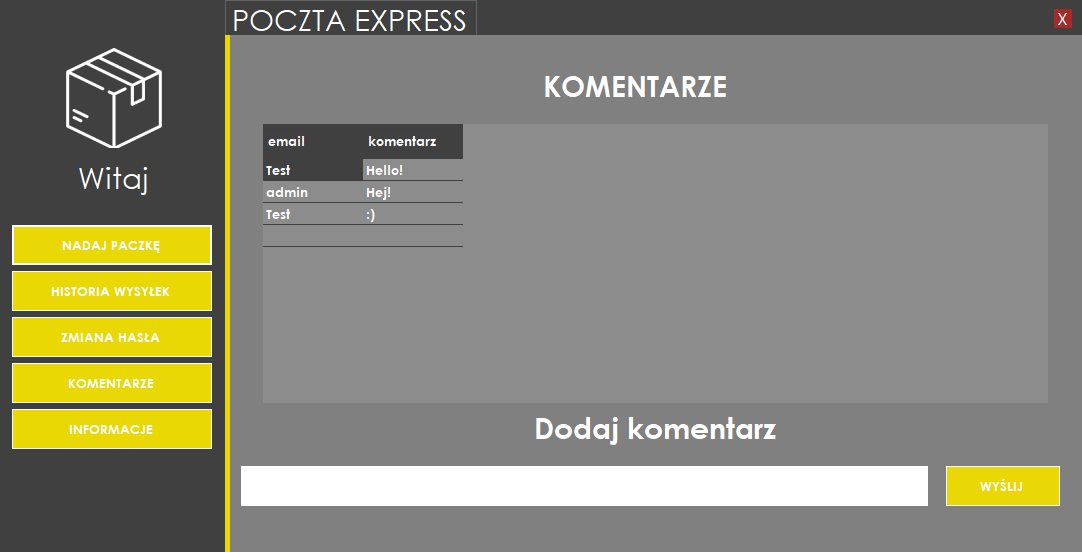
\includegraphics[width=16.5cm, height=9cm]{figures/komentarze.png}
\caption{\footnotesize Okno zawierające możliwość komentowania. }
\label{fig:plotend}
\end{figure}

\subsection{Informacje}

Okno (Rysunek14) wyświetla kontakt do administratora aplikacji oraz aktualną wersję aplikacji.

\begin{figure}[!ht]
\centering
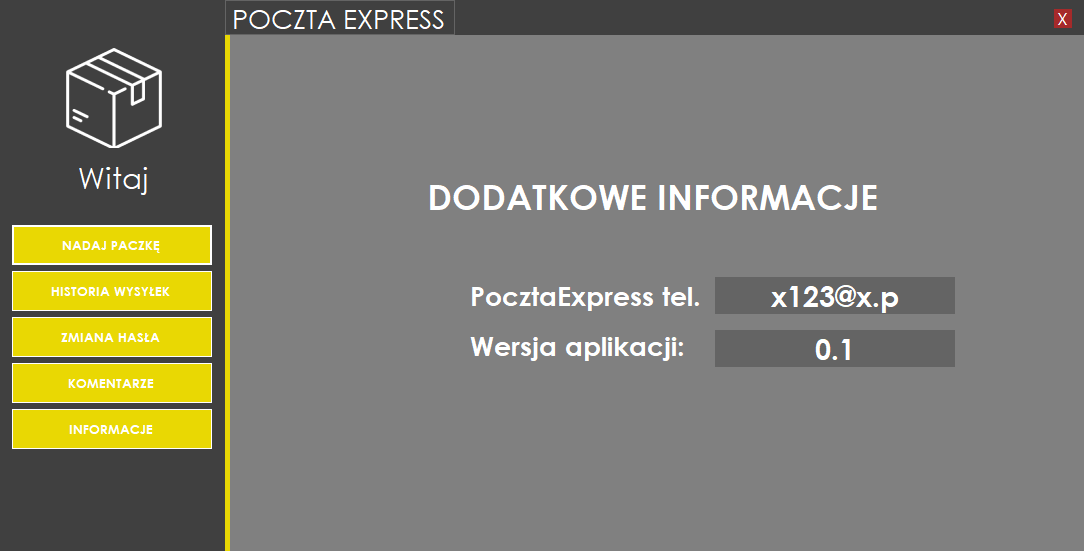
\includegraphics[width=16.5cm, height=9cm]{figures/informacje.png}
\caption{\footnotesize Okno zawierające informacje o aplikacji). }
\label{fig:plotend}
\end{figure}

\newpage
\subsection{Panel administratora}
Aplikacja zawiera również panel sterowania dostępny tylko dla administratora aplikacji (Rysunek 15). Po podaniu e-mailu, hasła administratora oraz zalogowaniu się, pojawi się okno z panelem dla administratora.
Panel zawiera listę paczek które zostały nadane od wszystkich użytkowników w aplikacji. Dodatkowo administrator ma możliwość zmiany aktualnych cen nadaniu przesyłki, ale również zmiany kontaktu oraz wersji w formie tekstowej które znajdują się w oknie dotyczące informacji o aplikacji.

\begin{figure}[!ht]
\centering
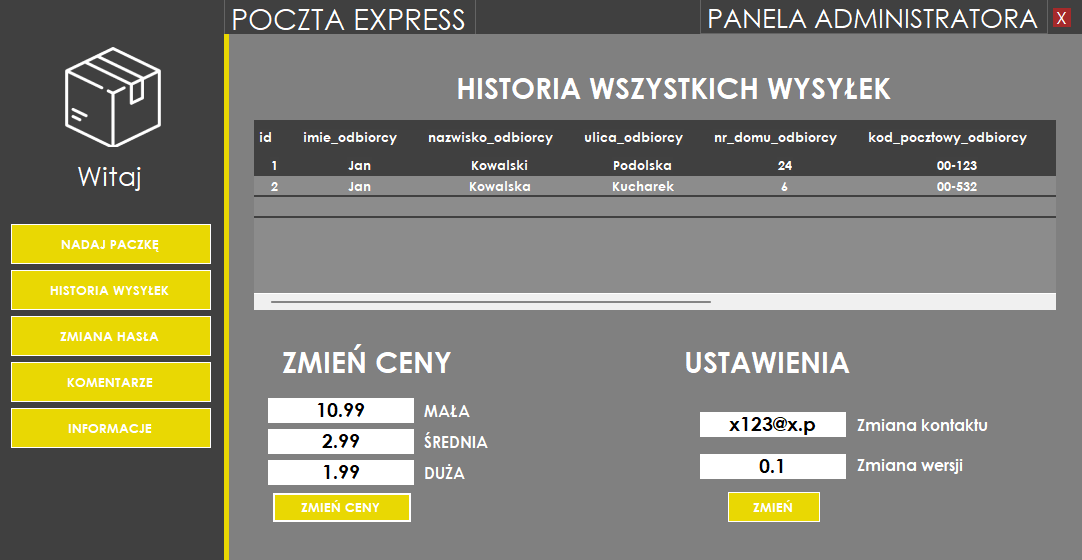
\includegraphics[width=16.5cm, height=9cm]{figures/admin.png}
\caption{\footnotesize Panel administratora}
\label{fig:plotend}
\end{figure}


\subsection{Zamknięcie aplikacji}

W każdym oknie aplikacji występuje ikona (Rysunek 16) umożliwiająca zamknięcie aplikacji

\begin{figure}[!ht]
\centering

\includegraphics[width=1.5cm, height=1.5cm]{figures/ikona zamkniecia.png}
\caption{\footnotesize Ikona umożliwiająca zamknięcie aplikacji. }
\label{fig:plotend}
\end{figure}
\newpage
\section{Podsumowanie}

W ramach projektu aplikacji PocztaExpress zrealizowano kluczowe funkcjonalności umożliwiające użytkownikom wygodne nadawanie przesyłek bez konieczności wizyty w placówkach pocztowych. Aplikacja obsługuje rejestrację użytkowników, historię wysyłek oraz podstawowe operacje logistyczne związane z nadawaniem paczek. System został zaprojektowany z myślą o intuicyjnym interfejsie użytkownika oraz kompatybilności z systemami Windows 10/11 i .NET 6.0.
\newline

\noindent Zrealizowane prace obejmowały:
\begin{itemize}
\item Opracowanie i implementację interfejsu użytkownika (okna logowania, formularz nadania paczki, historia przesyłek itp.).
\item Integrację z bazą danych do przechowywania informacji o przesyłkach i użytkownikach.
\item Implementację funkcji rejestracji, logowania oraz zarządzania kontem użytkownika.
\item Dodanie modułu zmiany hasła i sekcji kontaktowej.
\item Stworzenie systemu wyświetlania historii nadanych paczek.
\item Stworzenie systemu dodawania punktów do użytkownika
\item Możliwość dodania komentarzy
\end{itemize}

\noindent W przyszłości możliwe jest jej rozwinięcie o dodatkowe funkcjonalności, takie jak integracja z systemami ERP dla firm, automatyczne powiadomienia SMS dla odbiorców oraz obsługa międzynarodowych przesyłek, możliwość śledzenia przesyłek w czasie rzeczywistym, optymalizacja wydajności aplikacji oraz usprawnienie obsługi błędów, rozwój wersji mobilnej aplikacji na systemy Android oraz iOS, umożliwienie płatności online za wysłanie przesyłki Dzięki zastosowanym technologiom aplikacja jest nowoczesnym i efektywnym narzędziem do zarządzania procesem wysyłki paczek.


\newpage
\section{Literatura}

\noindent Microsoft Docs – Oficjalna dokumentacja: .NET 6 Documentation 
\newline
https://learn.microsoft.com/pl-pl/dotnet/csharp/language-reference - dokumentacja języka C\# | Microsoft Learn 




\end{document}
% *************** Koniec pliku szablon.tex ***************
